Cette partie est très importante dans le cycle de vie du projet. Théoriquement, toute la fondation du projet a été construite dans cette base, par la suite, il ne reste que la mise en œuvre.
	\section{Étude des données}
	\subsection{Règles de gestion recensées}
	Au cours de la réalisation du projet, j'ai vu qu’un ensemble de règles de gestion sont à respecter afin d'assurer la bonne satisfaction du besoin et le bon fonctionnement du système. Quant à ce projet j'ai proposé l’ensemble des règles suivantes:
	\begin{itemize}
		\item[•] L'administrateur de système doit demander l’accès au système pour recevoir les informations de son compte de part du directeur de l'espace Office 365 \textbf{DYN IT}.
		\item[•] L'administrateur doit choisir un contrat pour accéder et gérer ses informations.
		\item[•] L'administrateur doit voir toujours les informations d'entête d'un contrat sélectionné.
		\item[•] L'administrateur doit choisir un contrat et une période pour accéder et gérer les informations reliées aux avancements semestriels.
		\item[•] L'administrateur doit avoir un référentiel des délégants et des délégataires.
		\item[•] L'administrateur doit avoir la possibilité de modifié le référentiel des délégants ou des délégataires.
		\item[•] L'administrateur doit avoir la possibilité d'accéder à des tableaux de bord modifiable selon le contrat et/ou la période.
		\item[•] L'administrateur doit avoir la possibilité de générer des rapports d'un contrat et/ou une période sélectionnée.
	\end{itemize}
	\subsection{Dictionnaire des données}
	Pour bien comprendre les données traitées dans ce projet, j'ai obtenu plusieurs documents de suivi et un exemple de contrat de gestion déléguée. Ainsi, j'ai proposé le dictionnaire des données suivant. Ce dernier est divisées en plusieurs tableaux qui sont classées dans trois catégories:
	\begin{itemize}
		\item[•] Les données d'entête: Ils représentes les informations qui définissent un contrat. Certes, ils peuvent être gérer, mais ils ne dépendent pas des périodes. Ils ne peuvent pas être changées sauf dans le cadre d'une révision ou d'un avenant.
		\item[•] Les données des référentiels: Ils représentes les informations qui ne dépendent ni du contrat et ni de la période. En effet, il peuvent être inclus dans la définitions d'un contrat.
		\item[•] Les données d'avancements: Ils représentes les informations qui dépendent du contrat et de la période.
	\end{itemize}

	\subsubsection{• Les données d'entête}

	Cette catégorie groupe les données des contrats, des révisions, des avenants, des tarifs, etc.

	\begin{table}[H]
		\begin{center}
			\begin{tabularx}{17.5cm}{|p{3.5cm}|X|p{3.5cm}|}
				\hline
				\textbf{Attribut}    & \textbf{Signification}                                        & \textbf{Exemple}    \\
				\hline
				NumContrat           & Numéro du contrat                                             & 45858               \\
				\hline
				LibelleContrat       & Libellé du contrat                                            & ALBAIDA             \\
				\hline
				DateDemarrageContrat & Date de démarrage du contrat                                  & 01/11/2019          \\
				\hline
				DateFinContrat       & Date du fin du contrat                                        & 01/11/2027          \\
				\hline
				DateVisa             & Date visa                                                     & 01/06/2019          \\
				\hline
				DureeContrat         & Durée du contrat                                              & 10 ans              \\
				\hline
				Delegant             & Nom du délégant                                               & Commune Tanger      \\
				\hline
				Delegataire          & Nom du délégataire                                            & ALSA Tanger         \\
				\hline
				Autre Partenaire     & Nom d'un partenaire (autre que le délégant et le délégataire) & Coopération El-Amal \\
				\hline
				NumAvenant           & Numéro d'avenant                                              & 5245                \\
				\hline
				LibelleAvenant       & Libellé d'avenant                                             &                     \\
				\hline
				DateAvenant          & Date d'avenant                                                & 01/06/2023          \\
				\hline
				MotifAvenant         & Motif d'avenant                                               &                     \\
				\hline
				Status               & Status d'avenant                                              & Actif/ Non Actif    \\
				\hline
				NumRevision          & Numéro de révision                                            & 2336                \\
				\hline
				LibelleRevision      & Libellé de révision                                           &                     \\
				\hline
				DateRevision         & Date de révision                                              & 01/01/2026          \\
				\hline
				MotifRevision        & Motif de la révision                                          &                     \\
				\hline
			\end{tabularx}
			\caption{Table d'entête}
		\end{center}
	\end{table}
	\begin{table}[H]
		\begin{center}
			\begin{tabularx}{17.5cm}{|p{6.5cm}|X|p{2.1cm}|}
				\hline
				\textbf{Attribut}                    & \textbf{Signification}                                       & \textbf{Exemple} \\
				\hline
				NumCommunesDesservies                & Nombre de communes desservies                                & 10               \\
				\hline
				Population                           & Population                                                   & 100252           \\
				\hline
				LongueurReseau                       & Longueur du réseau                                           & 200 Km           \\
				\hline
				LongueurLignesUrbaines               & Longueur des lignes urbaines                                 & 130 Km           \\
				\hline
				LongueurLignesPeripheriques          & Longueur des lignes périphériques                            & 70km             \\
				\hline
				NombreLignes                         & Nombre des lignes                                            & 24               \\
				\hline
				PrixMinTarifScolaire                 & Prix minimal de tarif scolaire                               & 3 Dhs            \\
				\hline
				PrixMaxTarifScolaire                 & Prix maximal de tarif scolaire                               & 6 Dhs            \\
				\hline
				PrixMinTarifNormal                   & Prix minimal de tarif normal                                 & 4 Dhs            \\
				\hline
				PrixMaxTarifNormal                   & Prix maximal de tarif normal                                 & 5 Dhs            \\
				\hline
				PrixMinTarifConvention               & Prix maximal de tarif convention                             & 5 Dhs            \\
				\hline
				PrixMaxTarifConvention               & Prix maximal de tarif convention                             & 7 Dhs            \\
				\hline
				ValeurInvestissementContractuelDN    & Valeur d'investissement contractuel de délégant              & 150000 Dhs       \\
				\hline
				NombreBusContractuelDN               & Nombre des bus contractuel de délégant                       & 50               \\
				\hline
				NombreAbriBusContractuelDN           & Nombre des abris bus contractuel de délégant                 & 15               \\
				\hline
				NombreArretContractuelDN             & Nombre des arrêts contractuel de délégant                    & 150              \\
				\hline
				NombreAireStationnementContractuelDN & Nombre des aires de stationnement contractuel de délégant    & 10               \\
				\hline
				ValeurInvestissementContractuelDT    & Valeur d'investissement contractuelle de délégataire         & 100000 Dhs       \\
				\hline
				NombreBusContractuelDT               & Nombre des bus contractuel de délégataire                    & 45               \\
				\hline
				NombreAbriBusContractuelDT           & Nombre des abris bus contractuel de délégataire              & 10               \\
				\hline
				NombreArretContractuelDT             & Nombre des arrêts contractuel de délégataire                 & 120              \\
				\hline
				NombreAireStationnementContractuelDT & Nombre des aires de stationnement contractuel de délégataire & 7                \\
				\hline
			\end{tabularx}
			\caption{Suite 1 de la table d'entête}
		\end{center}
	\end{table}
	\begin{table}[H]
		\begin{center}
			\begin{tabularx}{17.5cm}{|p{6cm}|X|p{1.6cm}|}
				\hline
				\textbf{Attribut}                    & \textbf{Signification}                                                                                          & \textbf{Exemple} \\
				\hline
				ValeurInvestissementContractuelleAT  & Valeur d'investissement contractuelle des autres partenaires (autre que le délégants et le délégataire)         & 90000 Dhs        \\
				\hline
				NombreBusContractuelAT               & Nombre des bus contractuel des autres partenaires (autre que le délégants et le délégataire)                    & 30               \\
				\hline
				NombreAbriBusContractuelAT           & Nombre des abris bus contractuel des autres partenaires (autre que le délégants et le délégataire)              & 7                \\
				\hline
				NombreArretContractuelAT             & Nombre des arrêts contractuel des autres partenaires (autre que le délégants et le délégataire)                 & 80               \\
				\hline
				NombreAireStationnementContractuelAT & Nombre des aires de stationnement contractuel des autres partenaires (autre que le délégants et le délégataire) & 0                \\
				\hline
			\end{tabularx}
			\caption{Suite 2 de la table d'entête}
		\end{center}
	\end{table}

	\subsubsection{Les données des référentiels}

	Cette catégorie groupe les données des délégataires, des délégants et des communes.

	\begin{table}[H]
		\begin{center}
			\begin{tabularx}{17.5cm}{|p{3cm}|p{3cm}|X|}
				\hline
				\textbf{Attribut} & \textbf{Signification} & \textbf{Exemple}                                       \\
				\hline
				NomDelegant       & Nom du délégant        & Établissement de Coopération Intercommunal  "Al Baida" \\
				\hline
			\end{tabularx}
			\caption{Référentiel des délégants}
		\end{center}
	\end{table}

	\begin{table}[H]
		\begin{center}
			\begin{tabularx}{17.5cm}{|p{3cm}|p{3cm}|X|}
				\hline
				\textbf{Attribut} & \textbf{Signification} & \textbf{Exemple}    \\
				\hline
				NomDelegataire    & Nom du délégataire     & Société ALSA Tanger \\
				\hline
			\end{tabularx}
			\caption{Référentiel des délégataires}
		\end{center}
	\end{table}

	\newpage
	\subsubsection{Les données des avancements}

	Cette catégorie groupe les données d'effectif personnel, des investissements, des matériaux roulants et fixes, etc\dots


	\begin{table}[H]
		\begin{center}
			\begin{tabularx}{17.5cm}{|p{2.5cm}|X|p{2.5cm}|}
				\hline
				\textbf{Attribut} & \textbf{Signification}                                                                              & \textbf{Exemple} \\
				\hline
				numcontrat        & Numéro du Contrat                                                                                   & 25462            \\
				\hline
				numavenant        & Numéro d'avenant                                                                                    & 14528            \\
				\hline
				numrevision       & Numéro de révision                                                                                  & 1552             \\
				\hline
				valeur\_delegant  & Somme investi par le délégant                                                                       & 900000 Dhs       \\
				\hline
				abri\_delegant    & Nombre des abris bus de délégant                                                                    & 6                \\
				\hline
				arret\_delegant   & Nombre des arrêts de délégant                                                                       & 7                \\
				\hline
				bus\_delegant     & Nombre des bus de délégant                                                                          & 50               \\
				\hline
				air\_delegant     & Nombre des aires de stationnement de délégant                                                       & 30               \\
				\hline
				air\_delegataire  & Nombre des aires de stationnement de délégataire                                                    & 25               \\
				\hline
				valeur\_autre     & Somme investi par les autres partenaires (autre que le délégants et le délégataire)                 & 800000 Dhs       \\
				\hline
				abri\_autre       & Nombre des abris bus des autres partenaires (autre que le délégants et le délégataire)              & 3                \\
				\hline
				arret\_autre      & Nombre des arrêts des autres partenaires (autre que le délégants et le délégataire)                 & 25               \\
				\hline
				bus\_autre        & Nombre des bus des autres partenaires (autre que le délégants et le délégataire)                    & 20               \\
				\hline
				air\_autre        & Nombre des aires de stationnement des autres partenaires (autre que le délégants et le délégataire) & 15               \\
				\hline
				datedemiseajour   & Date de mise à jour                                                                                 & 16/04/2021       \\
				\hline
				periode           & Année/semestre                                                                                      & 2020/S1          \\
				\hline
			\end{tabularx}
			\caption{Table d'investissements réalisés}
		\end{center}
	\end{table}

	\begin{table}[H]
		\begin{center}
			\begin{tabularx}{17.5cm}{|X|X|p{2.5cm}|}
				\hline
				\textbf{Attribut}                  & \textbf{Signification}                     & \textbf{Exemple} \\
				\hline
				numcontrat                         & Numéro du Contrat                          & 25462            \\
				\hline
				numavenant                         & Numéro d'avenant                           & 14528            \\
				\hline
				numrevision                        & Numéro de révision                         & 1552             \\
				\hline
				abrisBusNombre                     & Nombre des abris bus                       & 15               \\
				\hline
				abrisBusAgeMoyen                   & Âge moyen de bus                           & 5 ans            \\
				\hline
				abrisBusSatisfaction               & Satisfaisante des abris bus                & 76\%             \\
				\hline
				abrisBusCapacitéTotale             & Capacité totale des abris bus              & 30 personnes     \\
				\hline
				arretsNombre                       & Nombre des arrêts                          & 50               \\
				\hline
				arretsAgeMoyen                     & Âge moyen des arrêts                       & 5 ans            \\
				\hline
				arretsSatisfaction                 & Satisfaisante des arrêts                   & 80\%             \\
				\hline
				arretsCapacitéTotale               & Capacité totale des arrêts                 & 15 personnes     \\
				\hline
				ateliersNombre                     & Nombre des ateliers                        & 3                \\
				\hline
				atelierAgeMoyen                    & Âge moyen des ateliers                     & 15 ans           \\
				\hline
				ateliersSatisfaction               & Satisfusance des ateliers                  & 70\%             \\
				\hline
				ateliersCapacitéTotale             & Capacité totale des ateliers               & 100 personnes    \\
				\hline
				airesDeStationnementNombres        & Nombre des aires de stationnement          & 45               \\
				\hline
				airesDeStationnementAgeMoyen       & Âge moyen des aires de stationnement       & 7 ans            \\
				\hline
				airesDeStationnementSatisfaction   & Satisfusance des aires de stationnement    & 77\%             \\
				\hline
				airesDeStationnementCapacitéTotale & Capacité totale des aires de stationnement & 70 personnes     \\
				\hline
				guichetNombre                      & Nombre des guichets                        & 50 guichets      \\
				\hline
				guichetAgeMoyen                    & Âge moyen des guichets                     & 7 ans            \\
				\hline
				guichetCapacitéTotale              & Capacité totale des guichets               & 10 personnes     \\
				\hline
				guichetSatisfaction                & Satisfusance des guichets                  & 63\%             \\
				\hline
				datedemiseajour                    & Date de mise à jour                        & 16/04/2021       \\
				\hline
				periode                            & Année/semestre                             & 2020/S1          \\
				\hline
			\end{tabularx}
			\caption{Table des matériaux fixes}
		\end{center}
	\end{table}

	\begin{table}[H]
		\begin{center}
			\begin{tabularx}{17.5cm}{|p{6cm}|X|p{2.5cm}|}
				\hline
				\textbf{Attribut}          & \textbf{Signification}                            & \textbf{Exemple} \\
				\hline
				numcontrat                 & Numéro du Contrat                                 & 25462            \\
				\hline
				numavenant                 & Numéro d'avenant                                  & 14528            \\
				\hline
				numrevision                & Numéro de révision                                & 1552             \\
				\hline
				BusStandardNombre          & Nombre des bus standard                           & 50               \\
				\hline
				busStandardAgeMoyen        & Âge moyen des bus standard                        & 7 ans            \\
				\hline
				busStandardKmParcourus     & Nombre des Km parcourus des bus standard          & 80 Km            \\
				\hline
				busArticuleNombre          & Nombre des bus articulés                          & 20               \\
				\hline
				busArticuleAgeMoyen        & Âge moyen des bus articulés                       & 7 ans            \\
				\hline
				busArticulesKmParcourus    & Nombre des Km parcourus des bus articulés         & 10500 Km         \\
				\hline
				buselectriqueNombre        & Nombre des bus électriques                        & 10               \\
				\hline
				buselectriqueAgeMoyen      & Âge moyen des bus électriques                     & 10 ans           \\
				\hline
				buselectriqueKmParcourus   & Nombre des Km parcourus des bus électriques       & 80000 Km         \\
				\hline
				busSitesPropresNombre      & Nombre des bus des sites propres                  & 15               \\
				\hline
				busSitesPropresAgeMoyen    & Âge moyen des bus des sites propres               & 15 ans           \\
				\hline
				busSitesPropresKmParcourus & Nombre des Km parcourus des bus des sites propres & 70000 Km         \\
				\hline
				datedemiseajour            & Date de mise à jour                               & 16/04/2021       \\
				\hline
				periode                    & Année/semestre                                    & 2020/S1          \\
				\hline
			\end{tabularx}
			\caption{Table des matériaux circulants}
		\end{center}
	\end{table}

	\begin{table}[H]
		\begin{center}
			\begin{tabularx}{17.5cm}{|p{4cm}|X|p{2.5cm}|}
				\hline
				\textbf{Attribut}         & \textbf{Signification}                                                                                        & \textbf{Exemple} \\
				\hline
				numcontrat                & Numéro du Contrat                                                                                             & 25462            \\
				\hline
				numavenant                & Numéro d'avenant                                                                                              & 14528            \\
				\hline
				numrevision               & Numéro de révision                                                                                            & 1552             \\
				\hline
				PQM                       & Plan de Maintenance Qualité                                                                                   & oui              \\
				\hline
				Reclamation               & Réclamations des usagers                                                                                      & 152              \\
				\hline
				EquipementsPointsArret    & Équipements des points d'arrêt                                                                                & Poteaux          \\
				\hline
				SAEV                      & Système d'information de type Systèmes d'Aide à l'Exploitation et
				à l'Information Voyageurs & non                                                                                                                              \\
				\hline
				SysGeo                    & Système de géolocalisation                                                                                    & oui              \\
				\hline
				AdresseSTR                & Site internet et information disponible en temps réel (adresse)                                               & non              \\
				\hline
				AdressedescpSTR           & Site internet et information disponible  en temps réel (Description d'adresse)                                & oui              \\
				\hline
				ReseauSTR                 & Site internet et information disponible  en temps réel (Informations Statiques sur le réseau)                 & oui              \\
				\hline
				ReseaudescpSTR            & Site internet et information disponible  en temps réel (Description des informations Statiques sur le réseau) & non              \\
				\hline
				HoraireServiceSTR         & Site internet et information disponible  en temps réel (Horaire du services)                                  & oui              \\
				\hline
				HoraireServicedescpSTR    & Site internet et information disponible  en temps réel (Description d'horaire du services)                    & oui              \\
				\hline
				PerturbationsSTR          & Site internet et information disponible  en temps réel (Informations sur les perturbations)                   & oui              \\
				\hline
				PerturbationsdescpSTR     & Site internet et information disponible  en temps réel (Description des informations sur les perturbations)   & oui              \\
				\hline
				TarifSTR                  & Site internet et information disponible  en temps réel (Tarifs appliqués)                                     & non              \\
				\hline
				TarifdescpSTR             & Site internet et information disponible  en temps réel (Description des tarifs appliqués)                     & oui              \\
				\hline
				VenteSTR                  & Site internet et information disponible  en temps réel(Vente en ligne)                                        & non              \\
				\hline
				VentedescpSTR             & Site internet et information disponible  en temps réel(Description des ventes en ligne)                       & oui              \\
				\hline
			\end{tabularx}
			\caption{Table de la qualité des services}
		\end{center}
	\end{table}
	\begin{table}[H]
		\begin{center}
			\begin{tabularx}{17.5cm}{|p{4cm}|X|p{2.5cm}|}
				\hline
				\textbf{Attribut}                       & \textbf{Signification}                                                 & \textbf{Exemple} \\
				\hline
				CorrespondanceSTR                       & Site internet et information disponible en temps réel (correspondance) & oui              \\
				\hline
				CorrespondancedescpSTR                  & Site internet et information disponible en temps
				réel (Description de la correspondance) & oui                                                                                       \\
				\hline
				IntermodalieSTR                         & Site internet et information disponible en temps réel intermodalité    & oui              \\
				\hline
				IntermodaliedescpSTR                    & Site internet et information disponible en temps
				réel (Description d'intermodalité)      & oui                                                                                       \\
				\hline
				wifi                                    & wifi embarqué                                                          & oui              \\
				\hline
				VideoSurveillance                       & Vidéo surveillance embarquée                                           & oui              \\
				\hline
				CentreAppel                             & Centre d'appel                                                         & oui              \\
				\hline
				datedemiseajour                         & Date de mise à jour                                                    & 16/04/2021       \\
				\hline
				periode                                 & Année/semestre                                                         & 2020/S1          \\
				\hline
			\end{tabularx}
			\caption{Suite de la table de la qualité des services}
		\end{center}
	\end{table}

	\begin{table}[H]
		\begin{center}
			\begin{tabularx}{17.5cm}{|p{4cm}|X|p{2cm}|}
				\hline
				\textbf{Attribut}    & \textbf{Signification}                           & \textbf{Exemple} \\
				\hline
				numcontrat           & Numéro du Contrat                                & 25462            \\
				\hline
				numavenant           & Numéro d'avenant                                 & 14528            \\
				\hline
				numrevision          & Numéro de révision                               & 1552             \\
				\hline
				NumVoyJrS            & Nombre moyen de voyageurs/jour  sur un semestre  & 15023            \\
				\hline
				NumPVJrS             & Nombre moyen place vide /jour  sur un semestre   & 1252             \\
				\hline
				VoyageurTotalS       & Total annuel des voyageurs  sur un semestre      & 1252535          \\
				\hline
				TicketsVendusT       & Tickets vendus/semestre totale                   & 1250535          \\
				\hline
				TicketsVendusSc      & Tickets vendus/semestre tarif scolaire           & 125325           \\
				\hline
				TicketsVendusN       & Tickets vendus/semestre tarif normal             & 925634           \\
				\hline
				TicketsVendusC       & Tickets vendus/semestre tarif conventions        & 65828            \\
				\hline
				KmParTS              & Km parcourus/semestre totale semestriel parcouru & 152360 Km        \\
				\hline
				KmParMoyenS          & Km parcourus/semestre moyenne par ligne          & 1253 Km          \\
				\hline
				KmParMoyenSTrajL     & Km parcourus/semestre trajet le plus long        & 10535 Km         \\
				\hline
				KmParMoyenSTrajCourt & Km parcourus/semestre trajet le plus court       & 1253 Km          \\
				\hline
				KmParMoyenSTempsMax  & Km parcourus/semestre temps max trajet           & 8526 Km          \\
				\hline
				KmParMoyenSTempsMin  & Km parcourus/semestre temps min trajet           & 4253 Km          \\
				\hline
			\end{tabularx}
			\caption{Table des aspects commerciaux}
		\end{center}
	\end{table}
	\begin{table}[H]
		\begin{center}
			\begin{tabularx}{17.5cm}{|p{4cm}|X|p{2cm}|}
				\hline
				\textbf{Attribut} & \textbf{Signification}                                            & \textbf{Exemple} \\
				\hline
				Frequence         & Fréquence moyenne de passage unité/heure                          & 20               \\
				\hline
				Vitesse           & Vitesse commerciale moyenne Durée moyenne des trajets bus         & 60 Km/h          \\
				\hline
				Ponctualite       & Ponctualité Écart moyen entre horaire contractuel et horaire réel & 60\%             \\
				\hline
				TauxRemplissage   & Taux moyen de remplissage                                         & 80\%             \\
				\hline
				TauxTransVide     & Taux de transport à vide                                          & 15\%             \\
				\hline
				Depart            & Horaires du départ du service                                     & 05:00            \\
				\hline
				HeureFin          & Horaires de fin du service                                        & 11:00            \\
				\hline
				Pannes            & Pannes des bus sur la voie publique                               & 200              \\
				\hline
				Accidents         & Accidents de circulation des bus                                  & 132              \\
				\hline
				DélaiEva          & Délai moyen d'évacuation des véhicules en panne                   & 25 min           \\
				\hline
				datedemiseajour   & Date de mise à jour                                               & 16/04/2021       \\
				\hline
				periode           & Année/semestre                                                    & 2020/S1          \\
				\hline
			\end{tabularx}
			\caption{Suite de la table des aspects commerciaux}
		\end{center}
	\end{table}

	\begin{table}[H]
		\begin{center}
			\begin{tabularx}{17.5cm}{|p{4cm}|X|p{3cm}|}
				\hline
				\textbf{Attribut}   & \textbf{Signification}                                       & \textbf{Exemple} \\
				\hline
				numcontrat          & Numéro du Contrat                                            & 25462            \\
				\hline
				numavenant          & Numéro d'avenant                                             & 14528            \\
				\hline
				numrevision         & Numéro de révision                                           & 1552             \\
				\hline
				ConsommationMoyStd  & Consommation moyenne par km et par type de bus standard      & 15263 tonnes     \\
				\hline
				ConsommationMoyArt  & Consommation moyenne par km et par type de bus articulé      & 15263 tonnes     \\
				\hline
				ConsommationMoyElec & Consommation moyenne par km et par type de bus électrique    & 15263 tonnes     \\
				\hline
				ConsommationMoySite & Consommation moyenne par km et par type de bus sites propres & 15263 tonnes     \\
				\hline
				ConsommationAnn     & Consommation carburant annuelle pour l'ensemble du parc      & 152630 tonnes    \\
				\hline
				ConsommationAnnEle  & Consommation totale en électricité annuelle                  & 1526003 Kwh      \\
				\hline
				Emissions           & Émissions Carbone  Co2                                       & 15263 tonnes     \\
				\hline
				datedemiseajour     & Date de mise à jour                                          & 16/04/2021       \\
				\hline
				periode             & Année/semestre                                               & 2020/S1          \\
				\hline
			\end{tabularx}
			\caption{Table de l’efficacité énergétique}
		\end{center}
	\end{table}

	\begin{table}[H]
		\begin{center}
			\begin{tabularx}{17.5cm}{|p{4cm}|X|p{2cm}|}
				\hline
				\textbf{Attribut}      & \textbf{Signification}            & \textbf{Exemple} \\
				\hline
				numcontrat             & Numéro du Contrat                 & 25462            \\
				\hline
				numavenant             & Numéro d'avenant                  & 14528            \\
				\hline
				numrevision            & Numéro de révision                & 1552             \\
				\hline
				Conducteurs            & Nombre des conducteurs            & 200              \\
				\hline
				controleur             & Nombre des contrôleurs            & 70               \\
				\hline
				mécanicier             & Nombre des mécaniciens            & 30               \\
				\hline
				personnelAdministratif & Nombre du personnel administratif & 50               \\
				\hline
				datedemiseajour        & Date de mise à jour               & 16/04/2021       \\
				\hline
				periode                & Année/semestre                    & 2020/S1          \\
				\hline
			\end{tabularx}
			\caption{Table d'effectif personnel}
		\end{center}
	\end{table}

	\subsection{Le modèle conceptuel des données}

	Le MCD est une représentation statique du système d’information.
	Il a pour but d’écrire de façon formelle les données qui seront utilisées par le système d’information.
	Il s’agit donc d’une représentation des données, facilement compréhensible.
	Le formalisme adopté par la méthode Merise pour réaliser cette description est basé sur les concepts « entités association ».
	D’après ce qui précède, on obtient le MCD est décomposé en trois parties, comme suivant:
	\begin{figure}[H]
		\begin{center}
			\fbox{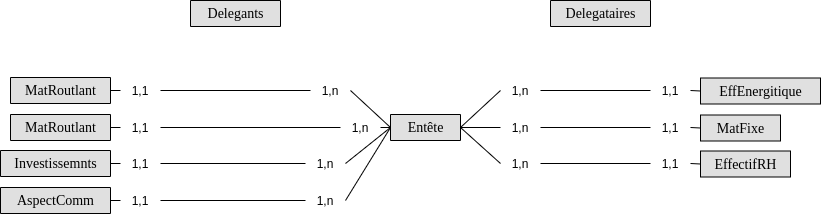
\includegraphics[scale=0.6]{MCD.png}}
			\caption{Le modèle conceptuel des données}
		\end{center}
	\end{figure}
	Suite à ce qui précède, j'ai proposé le schéma relationnel de la base de données, qui a été la base de la construction de cette dernière.

	\section{Diagramme des cas d'utilisation}
	\subsection{Gestion et suivi des contrats}

	La figure suivante est le DCU de gestion et le suivi d'un contrat. Ce dernier s’intègre
	dans le cadre d'UML. Il représente les possibilités d'interaction entre le système et les acteurs
	(intervenants extérieurs au système), c'est-à-dire de toutes les fonctionnalités que doit fournir le système.
	La figure suivante contient touts les cas d'interaction entre l'administrateur et le système concernant un contrat,
	à savoir chercher et consulter un contrat, chercher et consulter un agencement semestriel,
	ajouter un avenant, etc\dots
	\begin{figure}[H]
		\begin{center}
			\fbox{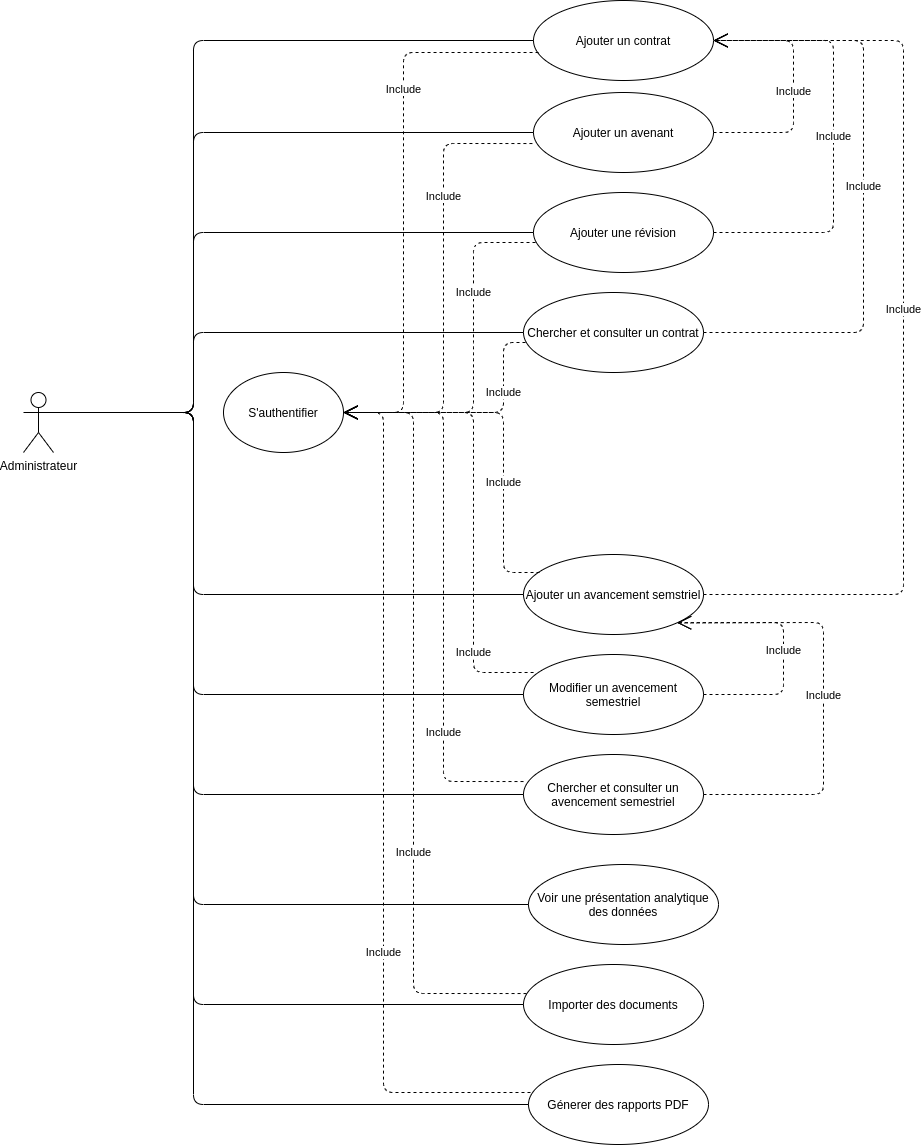
\includegraphics[scale=0.42]{UseCasesGestion-Suivi.png}}
			\caption{DCU:Gestion et suivi des contrats}
		\end{center}
	\end{figure}

	\subsection{Gestion des délégants}

	La figure suivante est le DCU de gestion des délégants.
	Elle contient touts les cas d'interaction entre l'administrateur et le système concernant un délégant,
	à savoir consulter la liste des délégants, chercher et modifier un délégant, et ajouter un délégant.
	\begin{figure}[H]
		\begin{center}
			\fbox{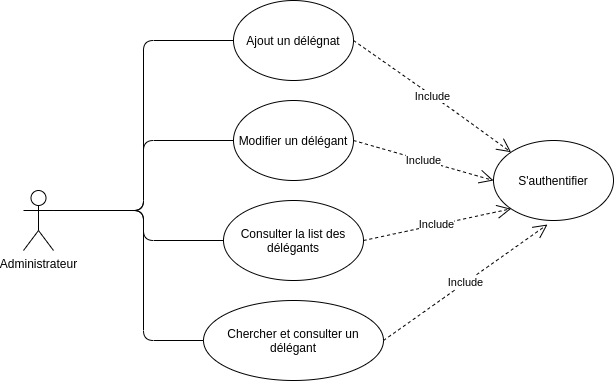
\includegraphics[scale=0.6]{UseCasesDelegants.png}}
			\caption{DCU:Gestion des délégants}
		\end{center}
	\end{figure}

	\subsection{Gestion des délégataires}

	La figure suivante est le DCU de gestion des délégataires.
	Elle contient touts les cas d'interaction entre l'administrateur et le système concernant un délégataire,
	à savoir consulter la liste des délégataires, chercher et modifier un délégataire, et ajouter un délégataire.
	\begin{figure}[H]
		\begin{center}
			\fbox{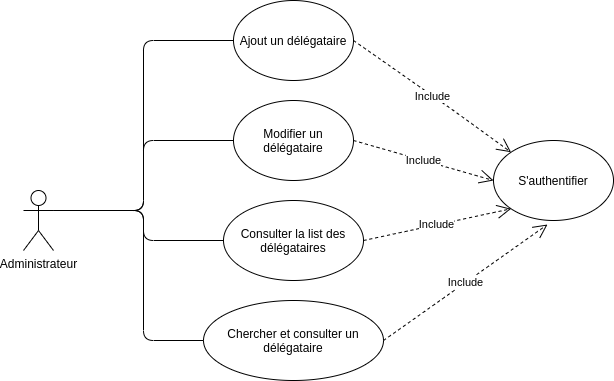
\includegraphics[scale=0.6]{UseCasesDelegatiares.png}}
			\caption{DCU:Gestion des délégataires}
		\end{center}
	\end{figure}

	\section{Modèle conceptuel des traitements}
	\subsection{Gestion et suivi des contrats}

	Dans le cadre de formalisme adopté par la méthode Merise, le MCT permet de représenter l’activité du
	système d’information d’une manière dynamique.
	Le schéma suivant représente le MCT de gestion et suivi des contrats. Parmi les traitements représentés
	on trouve la recherche et la consultation d'un contrat, d'un avancement semestriel,
	l'ajout d'un avenant, etc\dots

	\begin{figure}[H]
		\begin{center}
			\fbox{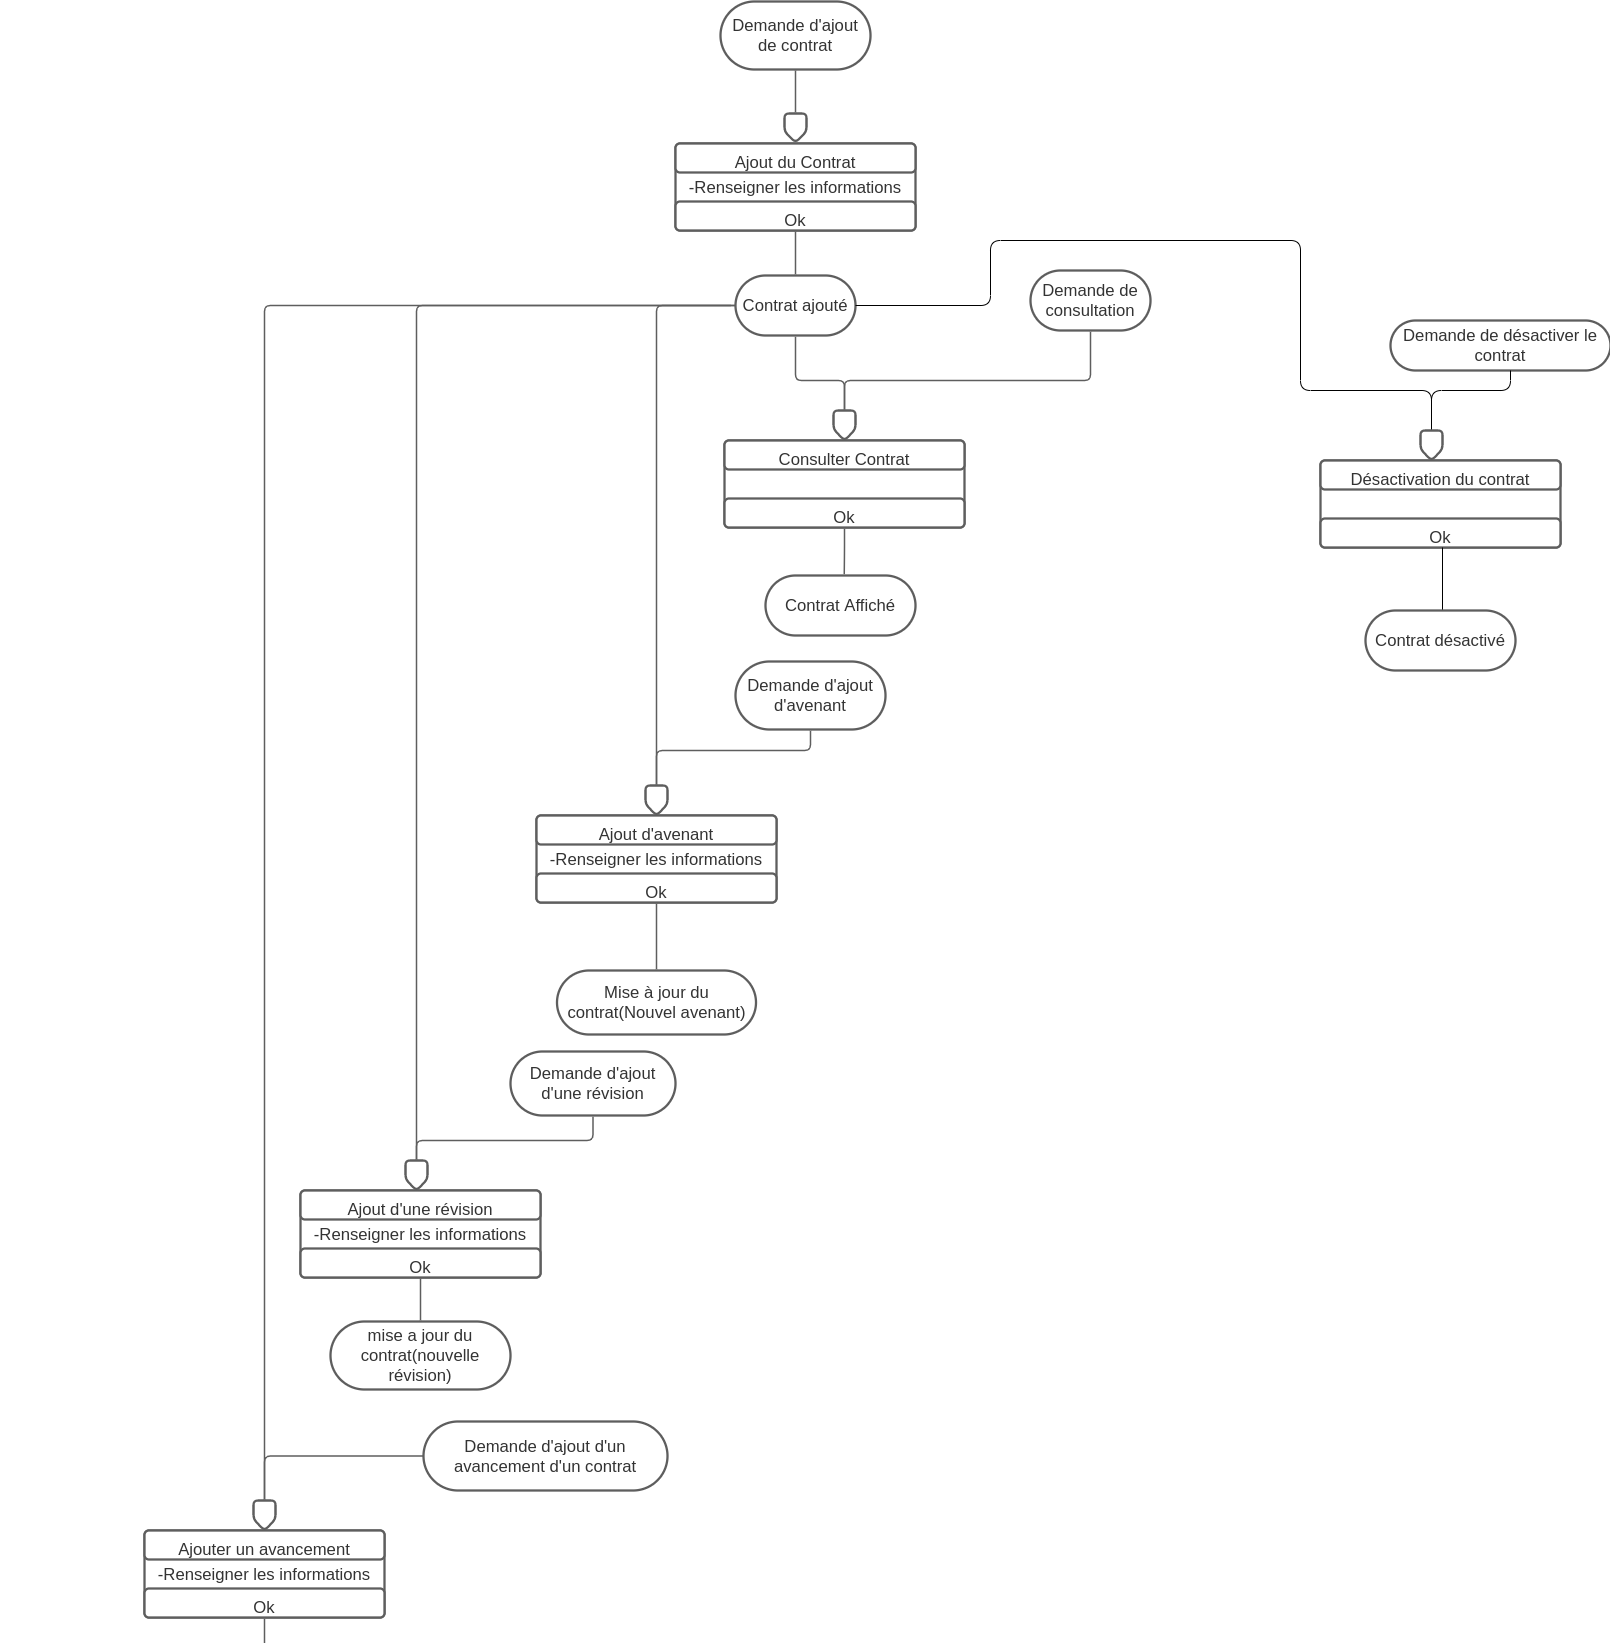
\includegraphics[scale=0.3]{MCT-Gestion-Suivi-1.png}}
			\caption{MCT:Gestion et suivi des contrats (partie contrat)}
		\end{center}
	\end{figure}

	\begin{figure}[H]
		\begin{center}
			\fbox{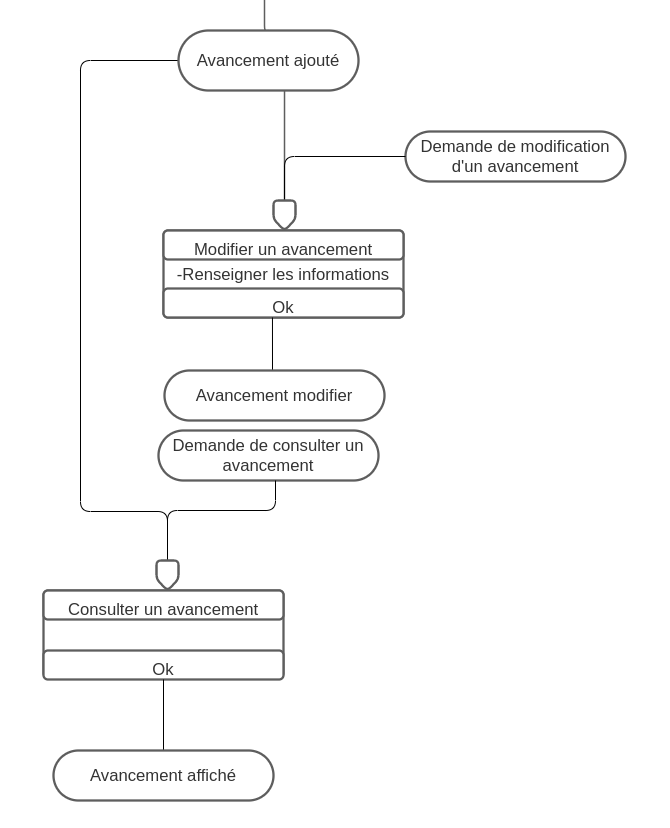
\includegraphics[scale=0.6]{MCT-Gestion-Suivi-2.png}}
			\caption{MCT:Gestion et suivi des contrats (partie avancement)}
		\end{center}
	\end{figure}

	\subsection{Gestion des délégants}

	Le schéma suivant représente le MCT de gestion des délégants. Parmi les traitements représentés
	on trouve la consultation de la liste des délégants, la recherche et la modification d'un délégant,
	et l'ajout d'un délégant.
	\begin{figure}[H]
		\begin{center}
			\fbox{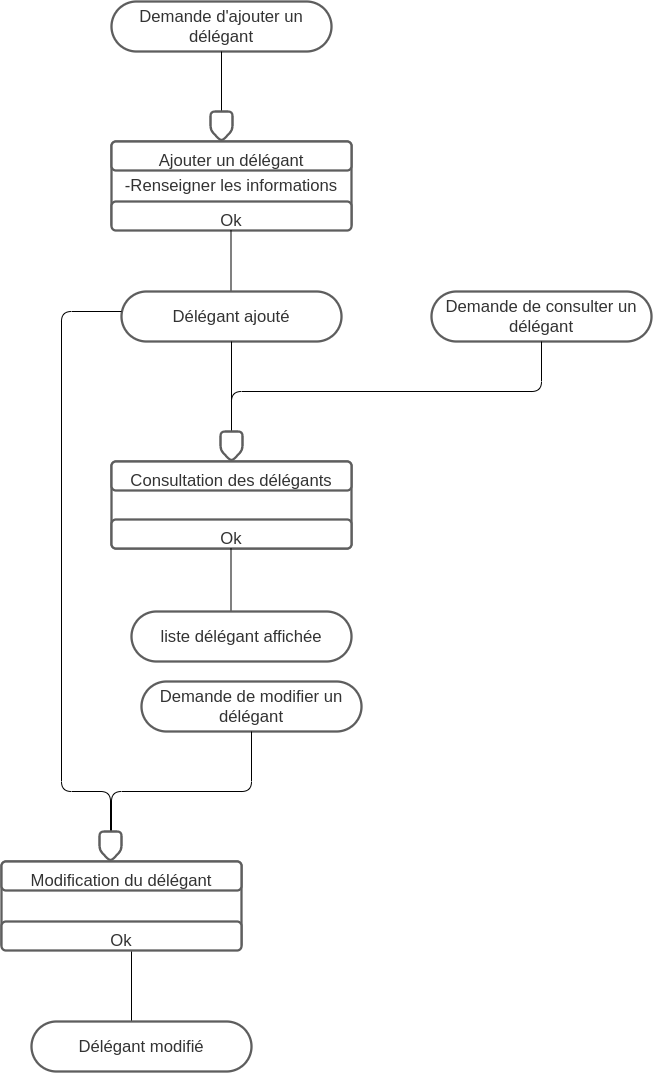
\includegraphics[scale=0.5]{MCT-Delegant.png}}
			\caption{MCT:Gestion des délégants}
		\end{center}
	\end{figure}

	\subsection{Gestion des délégataires}

	Le schéma suivant représente le MCT de gestion des délégataires. Parmi les traitements représentés
	on trouve la consultation de la liste des délégataires, la recherche et la modification d'un délégataire,
	et l'ajout d'un délégataire.
	\begin{figure}[H]
		\begin{center}
			\fbox{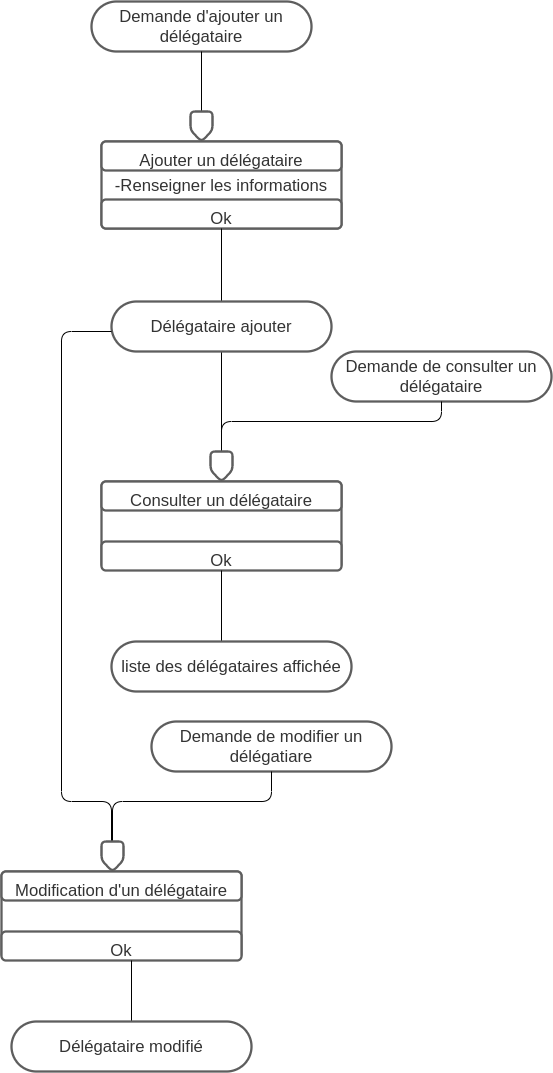
\includegraphics[scale=0.5]{MCT-Delegataire.png}}
			\caption{MCT:Gestion des délégataires}
		\end{center}
	\end{figure}

	\section{Les maquettes de l'application}

	Pour avoir une vue global de l'application, j'ai travaillé sur les maquettes suivantes. Il représente ma
	conception des écrans de l'application. Vous trouveriez dans la partie qui suit les maquettes principales
	de l'application:

	\subsection{Les écrans des contrats}

	En ce qui concerne un contrat, l'administrateur va avoir la possibilité de consulter la liste des contrats signés dans un tableau:
	\begin{figure}[H]
		\begin{center}
			\fbox{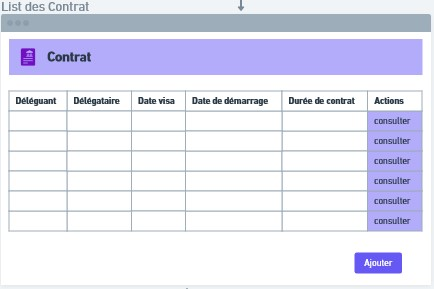
\includegraphics[scale=0.7]{maquette-7.jpeg}}
			\caption{Maquette de la liste des contrats}
		\end{center}
	\end{figure}

	Il peut également consulter un contrat sélectionné pour avoir les détails qu’en concerne dans un tableau:
	\begin{figure}[H]
		\begin{center}
			\fbox{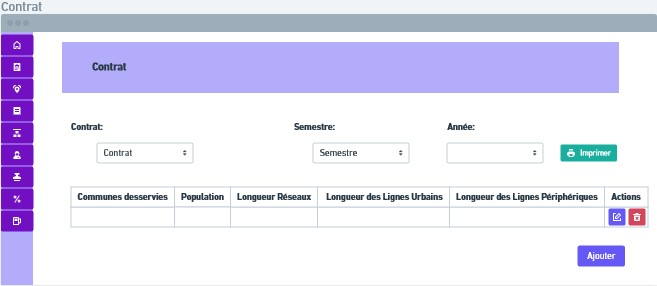
\includegraphics[scale=0.7]{maquette-2.jpeg}}
			\caption{Maquette de consultation d'un contrats}
		\end{center}
	\end{figure}

	Enfin, il peut ajouter un contrat en renseignant ses données dans un formulaire:
	\begin{figure}[H]
		\begin{center}
			\fbox{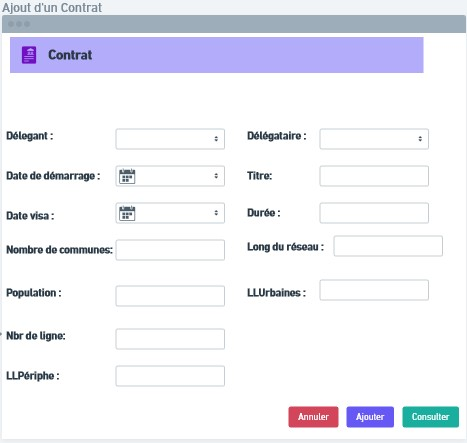
\includegraphics[scale=0.8]{maquette-4.jpeg}}
			\caption{Maquette d'ajout d'un contrat}
		\end{center}
	\end{figure}

	\subsection{Les écrans des avancements semestriels}

	Quant aux avancements semestriels, l'administrateur va avoir la possibilité
	de consulter les données d'une catégorie sélectionnée pour un contrat et une période définis:
	\begin{figure}[H]
		\begin{center}
			\fbox{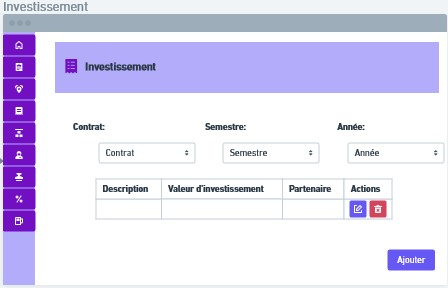
\includegraphics[scale=0.8]{maquette-1.jpeg}}
			\caption{Maquette de consultation d'un investissement}
		\end{center}
	\end{figure}

	De même que dans le cas d'un contrat, il peut ajouter une catégorie d'avancement en renseignant ses données dans un formulaire:
	\begin{figure}[H]
		\begin{center}
			\fbox{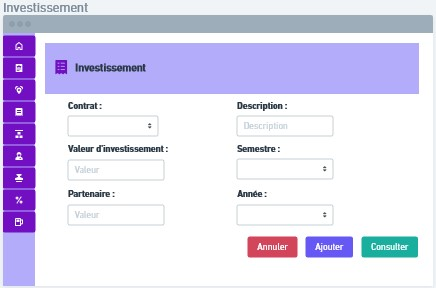
\includegraphics[scale=0.8]{maquette-9.jpeg}}
			\caption{Maquette d'ajout d'un avancement des investissements}
		\end{center}
	\end{figure}

	\begin{figure}[H]
		\begin{center}
			\fbox{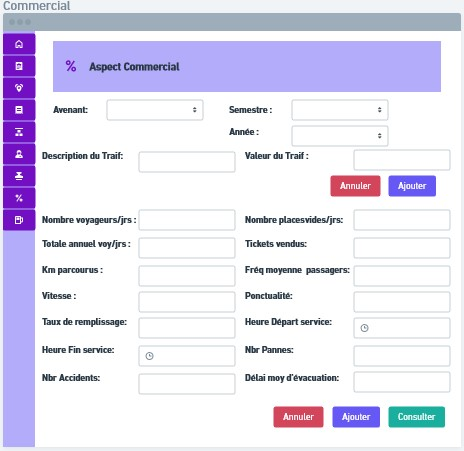
\includegraphics[scale=0.7]{maquette-3.jpeg}}
			\caption{Maquette d'ajout d'un avancement des aspects commerciaux}
		\end{center}
	\end{figure}

	\begin{figure}[H]
		\begin{center}
			\fbox{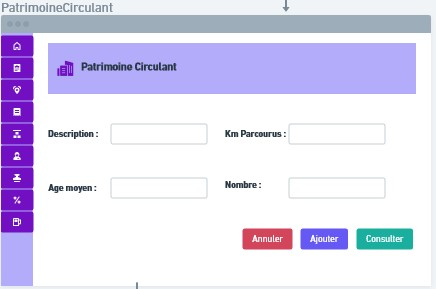
\includegraphics[scale=0.7]{maquette-5.jpeg}}
			\caption{Maquette d'ajout d'un avancement des matériaux circulants}
		\end{center}
	\end{figure}

	\begin{figure}[H]
		\begin{center}
			\fbox{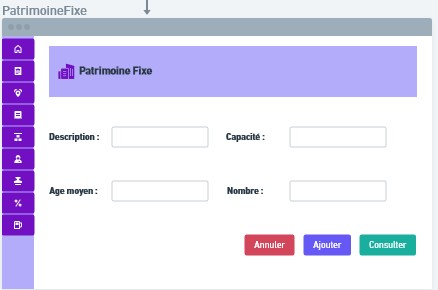
\includegraphics[scale=0.7]{maquette-6.jpeg}}
			\caption{Maquette d'ajout d'un avancement des matériaux fixes}
		\end{center}
	\end{figure}

	\section{Récapitulatif}

	Dans ce chapitre, j'ai préparé plusieurs diagrammes suivant les deux cadres de la méthode Merise et du langage UML.
	Autrement dite, tout ce qu’on a besoin pour l'élaboration de l’application. Dans le chapitre suivant,
	je vais mettre les mains dans la patte et présenter le projet réalisé.